\section{The band criterion}
\label{sec:band}

We use the parameters and the self-conjugate diagram $L$ from
\eqref{eq:candidate}, and write $K=2M-1$.  In particular,
$r=2b+s-1$.  The following criterion supplies constituents whose
diagrams have enough room for a path and its two attachments.

\begin{proposition}[Band criterion]\label{prop:band-test}
Let $M\ge9$, and let $\lambda\vdash |L|$ have column heights
$h_1\ge h_2\ge\cdots$ and row lengths $w_1\ge w_2\ge\cdots$,
with zeros appended.  Suppose that integers $d,q$ satisfy
$1\le d\le4$, $0\le q\le8$, and
\begin{equation}\label{eq:band-criterion}
 \sum_{i=1}^d w_i\ge K,\qquad
 dq+7+d\le K,\qquad
 \sum_{i=1}^q
      \max\left(0,\left\lfloor\frac{h_i-d}{2}\right\rfloor\right)
       \ge r.
\end{equation}
Then $S^\lambda$ occurs in $S^L\otimes S^L$.
\end{proposition}

The three inequalities have separate roles: the first gives room for
the path, the second reserves space at its endpoints, and the third
provides the even column heights needed for the attachments. We first
force the smaller cyclic triangle, then find nonzero path and attachment
contractions, and finally show that they combine without cancellation.
All alternating tensors use the conventions of
Section~\ref{sec:prelim}; changing the order of a block changes only its
overall sign.

\subsection{A forced triangle and a full induced quotient}

We first record the elementary induction fact used here and in the
balance constructions. It is the coordinate-sector principle of
\cite[Section~4]{SaxlCyclic}, applied to the marked alphabets of the
enlarged diagram.

\begin{lemma}[Induction from coordinate sectors]
\label{lem:sector-induction}
Let a finite group $G$ act transitively on a finite set $\Omega$.
Suppose a $G$-module has a direct-sum decomposition
$T=\bigoplus_{A\in\Omega}T_A$ with $gT_A=T_{gA}$.
Fix $D\in\Omega$, let $H$ be its stabilizer, and let $z\in T_D$.
Writing $A_0=\C[H]z$, the map
\[
 \C[G]\otimes_{\C[H]}A_0\longrightarrow\C[G]z,
 \qquad g\otimes a\longmapsto ga,
\]
is an isomorphism.  In particular, the cyclic module on the right is
the full induced module $\Ind_H^G A_0$.
\end{lemma}

\begin{proof}
Choose one representative $g_A$ with $g_AD=A$ for each $A\in\Omega$.
The source is the direct sum of the spaces $g_A\otimes A_0$.
Their images are $g_AA_0\subseteq T_A$, so the images for distinct
$A$ are linearly independent.  On each summand the displayed map is
injective, since $g_A$ acts invertibly.  Its image contains every
translate of $z$, proving surjectivity as well.
\end{proof}

Regard $L$ as its set $B$ of cells, with rows and columns indexed from
one.  Let $v_R,v_C$ be the alternating block tensors for its rows and
columns, respectively, and put
\[
 W_L=\C[S_B](v_R\otimes v_C).
\]
Both factors have type $L$, since $L$ is self-conjugate; hence
$W_L\subseteq S^L\otimes S^L$ after choosing the Specht
identifications.  Let
\[
 D=\{(i,j):i,j\ge1,\ i+j\le M-1\},\qquad F=B\setminus D.
\]
Thus $D$ is the staircase of order $M-2$, and
$|F|=K+2r$.

\begin{lemma}[Triangle quotient]\label{band:triangle-quotient}
There is a quotient of $W_L$ isomorphic to
\begin{equation}\label{eq:band-triangle-quotient}
 \Ind_{S_D\times S_F}^{S_B}
       (W_{M-2}\boxtimes U_F),
\end{equation}
where $W_{M-2}$ is the specified cyclic module in
Theorem~\ref{thm:cyclic-input}.  The module $U_F$ is generated by
the row and column block alternations on $F$, using an initial
alphabet on every remaining block.
Consequently, it suffices to find a diagram $\mu\subseteq\lambda$
of size $|F|$ such that $S^\mu$ occurs in $U_F$.
\end{lemma}

\begin{proof}
Set $\ell=M+b+s-1$, the largest row and column length of $L$.
The triangle $D$ has $t_i=\max(M-1-i,0)$ cells in row $i$
and in column $i$.  We will give each full row and column block
exactly this number of marked letters.
In each of the two alphabets $1,\ldots,\ell$, mark precisely
\[
 \{3,4,\ldots,M-1\}\cup\{M+b\}.
\]
There are $M-2$ marked letters.  The number of marked letters in
the initial alphabet of row or column $i$ is indeed $t_i$:
for the two largest blocks these counts are
$M-2,M-3$, and thereafter they are $M-4,M-5,\ldots,1,0,\ldots$.
The ordered unmarked alphabet is
$(1,2,M,\ldots,M+b-1)$, followed by $M+b+1$ if $s=2$.
The interval $M,\ldots,M+b-1$ is empty when $b=0$; in this case
the marked alphabet is $(3,\ldots,M)$ and the unmarked alphabet
is $(1,2)$ or $(1,2,M+1)$, respectively.  In every case each
block inherits an initial list in each of these two ordered
alphabets.
Project the pair-letter tensor space by retaining only those words
whose two letters at every position have the same marking status.
The projection commutes with permutations of positions.

For any retained term of $v_R\otimes v_C$, the set $A$ of marked
positions has row and column margins $(t_i)$.  For every $k$,
\[
 \sum_{i=1}^k t_i=\sum_j\min(k,t_j).
\]
Column $j$ can place at most $\min(k,t_j)$ marked cells in the
first $k$ rows.  Equality of the sums therefore gives equality in
every column.  Taking $k=t_j$ shows that, when $t_j>0$, all its
marked cells occupy the first $t_j$ rows.  Hence $A=D$.

Within each row or column block, the marked and unmarked positions
are now fixed.  Expanding that block's alternation gives the tensor
product of its marked and unmarked alternations, multiplied by one
fixed shuffle sign.  The two alphabets, each in its inherited order,
have initial lists on every block.  Thus, up to an overall sign, the
projected generator is
\[
 w_{M-2}\otimes u_F,
\]
where $w_{M-2}$ is exactly the row-column generator of
Theorem~\ref{thm:cyclic-input}, with its ordered alphabet relabeled,
and $u_F$ is the generator described in the statement.
The stabilizer $S_D\times S_F$ generates
$W_{M-2}\boxtimes U_F$ from this tensor.  To specify the sectors,
let $V_{\mathrm{mark}}$ and $V_{\mathrm{unmark}}$ be the pair-letter
spaces in which both letters are marked or both are unmarked,
respectively.  For $A\subseteq B$ with $|A|=|D|$, put
\[
 T_A=V_{\mathrm{mark}}^{\otimes A}\otimes
          V_{\mathrm{unmark}}^{\otimes(B\setminus A)}.
\]
These spaces have disjoint word bases, and $gT_A=T_{gA}$.
Lemma~\ref{lem:sector-induction} therefore identifies the entire
projected cyclic image with the full induced module in
\eqref{eq:band-triangle-quotient}, not merely with one of its
quotients.

For the last assertion, suppose $\mu\subseteq\lambda$.
Iterated branching implies that $S^\mu$ occurs on restriction of
$S^\lambda$ to $S_F$.  Decompose
$\Res_{S_D\times S_F}^{S_B}S^\lambda$ and then forget the $S_D$
action.  The occurrence just noted implies that some
$\alpha\vdash|D|$ satisfies $c_{\alpha,\mu}^{\lambda}>0$.
Theorem~\ref{thm:cyclic-input} supplies $S^\alpha$ in $W_{M-2}$.
Thus $S^\lambda$ occurs in the induced module in
\eqref{eq:band-triangle-quotient}, and hence in $W_L$ by complete
reducibility.
\end{proof}

\subsection{The path and its two attachments}

Write $\delta=s-1\in\{0,1\}$ and $E=(b+\delta,b)$, omitting
zero parts.  Each copy of $E$ has area $r$.
To decompose $F$, start with the boundary cells $i+j=M$ or $M+1$
in the staircase $B_M$.  They form a width-two path of length $K$.
Move its endpoint singletons from $(M,1)$ and $(1,M)$ to
$(\ell,1)$ and $(1,\ell)$, respectively.  More precisely, the
resulting path positions are $p_1,\ldots,p_K$, where
\begin{align*}
 p_1&=(\ell,1),&p_K&=(1,\ell),\\
 p_{2j}&=(M-j,j) &&(1\le j<M),\\
 p_{2j-1}&=(M+1-j,j) &&(2\le j<M).
\end{align*}
The northeastern attachment is
\[
 E_+=\{(1,j):M\le j\le\ell-1\}
       \cup\{(2,j):M\le j\le M+b-1\},
\]
with an interval interpreted as empty when its upper endpoint is
smaller than its lower endpoint.  Let $E_-$ be its transpose.
These sets are pairwise disjoint and exhaust $F$.
The attachment $E_+$ has shape $E$, and $E_-$ has the transposed
incidence pattern.

Along the path, the column pairs are
$(p_1,p_2),(p_3,p_4),\ldots,(p_{K-2},p_{K-1})$, with a column
singleton at $p_K$.  The row pairs are
$(p_2,p_3),(p_4,p_5),\ldots,(p_{K-1},p_K)$, with a row singleton
at $p_1$.  Only the first two column pairs and the last two row
pairs belong to blocks extended by attachment cells.

\begin{figure}[ht]
\centering
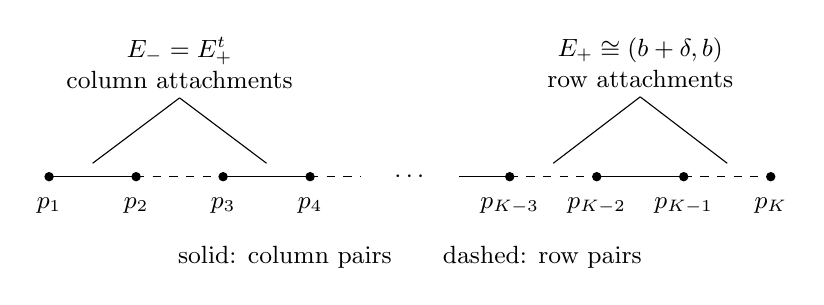
\begin{tikzpicture}[x=1.3cm,y=1cm, every node/.style={font=\small}]
 \foreach \name/\x/\lab in
   {a/0/{p_1},b/.85/{p_2},c/1.7/{p_3},d/2.55/{p_4},
    e/4.5/{p_{K-3}},f/5.35/{p_{K-2}},g/6.2/{p_{K-1}},h/7.05/{p_K}}
  {\coordinate (\name) at (\x,0);
   \fill (\name) circle (1.7pt);
   \node[below=4pt] at (\name) {$\lab$};}
 \draw (a)--(b); \draw[dashed] (b)--(c); \draw (c)--(d);
 \draw[dashed] (d)--(3.05,0);
 \node at (3.52,0) {$\cdots$};
 \draw (4,0)--(e);
 \draw[dashed] (e)--(f); \draw (f)--(g); \draw[dashed] (g)--(h);
 \node[align=center] (sw) at (1.275,1.45)
     {$E_-=E_+^t$\\column attachments};
 \draw (sw.south)--(.425,.17);
 \draw (sw.south)--(2.125,.17);
 \node[align=center] (ne) at (5.775,1.45)
     {$E_+\cong(b+\delta,b)$\\row attachments};
 \draw (ne.south)--(4.925,.17);
 \draw (ne.south)--(6.625,.17);
 \node at (3.525,-1.02)
     {solid: column pairs\qquad dashed: row pairs};
\end{tikzpicture}
\caption{Block-incidence schematic for $F$.  Each attachment extends
the two indicated pair blocks by $b+\delta$ and $b$ cells, respectively
(at the right, the outer pair receives $b+\delta$).
The displayed coordinates $p_i$ are defined in the text; the drawing
is not a geometric placement of the Young diagram.  Every path position
outside its first and last four belongs only to unextended blocks.}
\label{fig:band-attachments}
\end{figure}

Relabel the unmarked alphabet in increasing order, starting at one.
Let $P$ be the four-dimensional pair-letter space spanned by
$e_a\otimes e_c$ with $a,c\le2$.  Let
\[
 X_+=\Span\{e_a\otimes e_c:a>2,\ c\le2\},\qquad
 X_-=\Span\{e_a\otimes e_c:a\le2,\ c>2\},\qquad
 X=X_+\oplus X_-.
\]
Only letters available in the complement alphabet are included in
these spans.  There are $b+\delta$ letters above two, so
\[
 \dim X=4(b+\delta)\ge 4b+2\delta=2r.
\]
In particular, every extra diagram of size $2r$ fits this actual
alphabet; when $r=0$, both the diagram and $X$ are empty.
No cell of $F$ is simultaneously in one of its two long rows and
one of its two long columns, so every pair letter in $u_F$ lies in
$P\oplus X$.

\begin{lemma}[Separated contraction]\label{band:separated}
Retain from $u_F$ only terms using $P$ on the path, $X_+$ on $E_+$,
and $X_-$ on $E_-$.  The resulting tensor is, up to one nonzero
overall sign,
\begin{equation}\label{eq:band-separated}
 u_{\mathrm{path}}\otimes z_+\otimes z_-.
\end{equation}
Here $u_{\mathrm{path}}$ is the product of the two path block
alternations, with both endpoint singleton letters equal to one.
The tensors $z_+,z_-$ are the row-column alternating generators
for the two copies of $E$, with the long-block index shifted by two
and the two tensor layers interchanged for $E_-$.
\end{lemma}

\begin{proof}
In each extended block its two path positions must take its low
letters $1,2$, while its extra positions must take all remaining
letters.  These are prescribed sets of positions.  The alternation
therefore splits into an independent alternation on each set, with
a fixed shuffle sign.  Every other block belongs entirely to the
path or to one attachment.  Multiplying these factorizations proves
\eqref{eq:band-separated}.
\end{proof}

The selection in Lemma~\ref{band:separated} refers to fixed regions
of $F$ and need not commute with position permutations.
We will use the factorization inside a dual-polytabloid contraction:
the endpoint placement in the final proof will force precisely these
selected terms to survive.

\subsection{Contractions on an odd path}

For $t\ge0$, Brown, van Willigenburg, and Zabrocki
\cite[Corollary~4.1]{BWZ} proved that the square of $S^{(t+1,t)}$
contains exactly the partitions of $2t+1$ with at most four rows,
each with multiplicity one.  We need this support in a specified
cyclic path tensor, with any consecutive placement of the dual
columns.  The following proof extends the explicit contraction in
\cite[Section~5]{SaxlCyclic} to every odd length, including a single
position, and gives the common-basis conclusion needed for several
paths at once in the balance constructions.

\begin{lemma}[Odd-path support]\label{band:path-support}
Let $k=2t+1$ with $t\ge0$.  On positions $1,\ldots,k$, put
alternating pairs in the first layer on
$(2,3),(4,5),\ldots,(k-1,k)$ and the singleton letter $1$ at
position $1$.  In the second layer put alternating pairs on
$(1,2),(3,4),\ldots,(k-2,k-1)$ and the singleton letter $1$ at
position $k$.  Denote the resulting pair-letter tensor by $u$.

For every ordered list $a_1,\ldots,a_c$ with
$1\le a_i\le4$ and $\sum_i a_i=k$, place the columns of a dual
polytabloid consecutively along the path with these lengths.
There is a common ordered basis of $\Mat_2(\C)$ for which its
contraction with $u$ is nonzero.  In particular, the cyclic span of
$u$ contains every partition of $k$ with at most four rows.
For any finite collection of such paths and ordered column lists,
one common generic basis makes all their contractions nonzero.
\end{lemma}

\begin{proof}
Identify a pair-letter covector with a matrix $Y$ by evaluation
$Y(e_a\otimes e_c)=Y_{ac}$, and put
\[
 J=\begin{pmatrix}0&1\\-1&0\end{pmatrix}.
\]
Expanding the pair alternations and successively contracting the
indices along the path gives
\begin{align}
 \langle u,Y_1\otimes\cdots\otimes Y_k\rangle
 &=\bigl[Y_1JY_2^{\mathsf T}JY_3\cdots
                 JY_{k-1}^{\mathsf T}JY_k\bigr]_{11}\notag\\
 &=(-1)^t
   \bigl[Y_1\adj(Y_2)Y_3\cdots\adj(Y_{k-1})Y_k\bigr]_{11},
 \label{eq:band-path-contraction}
\end{align}
because $JY^{\mathsf T}J=-\adj(Y)$ for a two-by-two matrix.
The formula also holds for $k=1$, with no intervening factors.

Use the ordered matrix basis
\[
 M_1=I,\qquad
 M_2=Z=\begin{pmatrix}1&0\\0&-1\end{pmatrix},\qquad
 M_3=T=\begin{pmatrix}0&1\\1&0\end{pmatrix},\qquad M_4=J=ZT.
\]
The last three matrices are traceless, invertible, and pairwise
anticommuting.  Adjugation fixes $I$ and negates the other three.
For a segment of length $a\le4$ beginning at global position $p$,
write $D_j(Y)=Y$ for odd $j$ and $D_j(Y)=\adj(Y)$ for even $j$.
Its alternated matrix is
\[
 A_{a,p}=\sum_{\pi\in S_a}\sgn(\pi)
       D_p(M_{\pi(1)})\cdots D_{p+a-1}(M_{\pi(a)}).
\]
Let $e$ be the number of even positions in this segment, and let
$\epsilon=1$ when $p$ is even and $\epsilon=0$ otherwise.  Then
\begin{equation}\label{eq:band-segment}
 A_{a,p}=a!(-1)^{e-\epsilon}M_1\cdots M_a.
\end{equation}
Indeed, if $I$ occupies the local slot $j$, moving it there
contributes $(-1)^{j-1}$ to the permutation sign, while reordering
all remaining matrices contributes precisely their permutation
sign by anticommutation.  The adjugations contribute
$(-1)^{e-\epsilon_j}$, where $\epsilon_j$ records whether
$p+j-1$ is even.  Since
$\epsilon_j\equiv\epsilon+j-1\pmod2$, the total sign is
$(-1)^{e-\epsilon}$ for every summand.  This proves
\eqref{eq:band-segment}, whose right side is invertible.
For example, at length three the formula gives $-6J$ for both
starting parities: the canonical product is $IZT=J$, and
$e-\epsilon=1$ in either case.

Consequently, alternating independently within the prescribed
consecutive segments in \eqref{eq:band-path-contraction} gives
$(-1)^t[B]_{11}$, where $B$ is the ordered product of their
invertible matrices $A_{a,p}$.  Choose an eigenvector of $B$ with
nonzero eigenvalue $\beta$, and a matrix $Q\in\GL_2(\C)$ taking
it to the first coordinate vector.  Replace every $M_i$ by
$QM_iQ^{-1}$.  Since adjugation commutes with conjugation, the
new contraction is $(-1)^t[QBQ^{-1}]_{11}=(-1)^t\beta\ne0$.
The endpoint letters of $u$ have remained fixed throughout.

The dual tensor is a polytabloid for the partition with the
specified column lengths, regardless of their order along the
path.  Lemma~\ref{lem:dual-test} proves the support assertion.
For any one placement its contraction is a polynomial in the
entries of the common basis and is not identically zero by what
we just proved.  The nonvanishing loci of finitely many such
polynomials have nonempty intersection with the open set of
ordered bases, since $\GL_4(\C)$ is irreducible.  This proves the
last assertion.
\end{proof}

\subsection{The support of the two extra copies}

The path supplies the four-row component. We now determine enough
support in each attachment to supply every even-column diagram required
by the last inequality of Proposition~\ref{prop:band-test}.
The first step adapts the signed-average argument of
\cite[Section~3]{SaxlCyclic} to the two-row attachment.

\begin{lemma}[One extra copy]\label{band:one-extra}
Let $E=(b+\delta,b)$, where $b\ge0$ and $\delta\in\{0,1\}$,
and let $Z_E$ be the cyclic span of its row-column alternating
generator.  The sign twist $Z_E\otimes\sgn$ contains every
partition $\alpha\vdash 2b+\delta$ with at most four rows such
that all its row lengths are even when $\delta=0$, or exactly one
row length is odd when $\delta=1$.
\end{lemma}

\begin{proof}
The empty diagram is immediate, so assume $|E|>0$.
Let $p$ be its short-column alternating vector and $v$ its
long-row alternating vector.  These generate Specht modules of
types $E$ and $E^t$, respectively; denote them by
$V_p$ and $V_v$.  Put $G=S_{|E|}$ and $\varepsilon=\sgn$.
Let $H$ permute
positions within each short column, so that $hp=\sgn(h)p$.
Signed averaging of the product gives
\[
 \sum_{h\in H}\sgn(h)h(v\otimes p)
       =\left(\sum_{h\in H}hv\right)\otimes p.
\]
The first factor $v_0=\sum_{h\in H}hv$ is nonzero.  In fact the
word assigning letter $j$ to every cell of short column $j$ is
fixed by $H$ and has coefficient one in the row alternation $v$,
so its coefficient in $v_0$ is $|H|$.

Choose an abstract $G$-isomorphism
$\phi:V_v\otimes\varepsilon\longrightarrow V_p$, which exists
by sign conjugacy.  The $H$-alternating line of $V_p$ is unique:
\begin{align*}
 \dim\Hom_H(\varepsilon|_H,\Res_H^G V_p)
 &=\dim\Hom_G(\Ind_H^G\varepsilon|_H,V_p)\\
 &=\dim\Hom_G(\Ind_H^G\mathbf1,V_p\otimes\varepsilon)\\
 &=1.
\end{align*}
For the last equality, $H$ has block sizes given by $E^t$, and
$V_p\otimes\varepsilon\cong S^{E^t}$; this is the diagonal
multiplicity in Lemma~\ref{lem:young-support}.
Since $v_0$ is $H$-fixed,
$\phi(v_0\otimes\zeta)=cp$ for a nonzero sign-module vector
$\zeta$ and some $c\ne0$.  Reassociating the sign twist into
the first factor and then applying $\phi\otimes\mathrm{id}$
identifies $(V_v\otimes V_p)\otimes\varepsilon$ with
$V_p\otimes V_p$.  The image of $Z_E\otimes\varepsilon$
contains $cp\otimes p$, so it contains the cyclic span of
$p\otimes p$.

This is an isomorphism of abstract symmetric-group modules; it
does not change the physical long alphabet into a two-letter
alphabet.  It proves a support inclusion for the original
attachment module.  The subsequent contraction calculation may
therefore be made in the convenient realization of $p\otimes p$
on two copies of a two-dimensional alphabet.

Regroup the latter tensor by positions.  Each repeated short pair
is the symmetric tensor
\begin{equation}\label{eq:band-pair-form}
 H_0=e_{11}\otimes e_{22}+e_{22}\otimes e_{11}
       -e_{12}\otimes e_{21}-e_{21}\otimes e_{12}
\end{equation}
on the four-dimensional space with basis
$e_{ac}=e_a\otimes e_c$.  It is nondegenerate.  If $\delta=1$,
there is also the singleton vector $v_*=e_{11}$.

Suppose first that $\alpha$ has even rows.  Pair adjacent columns
of its dual tableau; the two columns in each pair have equal
height.  Place the $b$ position pairs of $H_0^{\otimes b}$
across corresponding rows of these paired columns.  Choose an
orthonormal basis of covectors for the form $H_0$.
In any nonzero term of the dual column alternations, the two
permutations on a paired column pair must match.  Their signs
therefore multiply to one.  A paired column pair of height $a$
contributes $a!$, so the entire contraction is nonzero.

When $\alpha$ has exactly one odd row, adjacent columns have
equal heights except for a single paired column pair of heights
$a,a-1$.  Put the singleton at the bottom of its longer column
and place the remaining position pairs across corresponding
rows.  In that exceptional pair, matching the other covectors
forces the singleton to receive the $a$th basis covector.
The contribution is $(a-1)!$ times its evaluation on $v_*$.
Choose the orthonormal basis so that this evaluation is nonzero;
this is possible since $v_*\ne0$, by permuting the members of
any orthonormal basis if necessary.  The covectors span the dual
space, so at least one evaluates nontrivially on $v_*$.  The other
column pairs contribute their positive factorials as before.  Thus this
contraction is also nonzero.  The height bound four ensures that
all covectors used belong to the available basis.
Lemma~\ref{lem:dual-test} completes the proof.
\end{proof}

\begin{lemma}[Two extra copies]\label{band:two-extras}
The cyclic span of $z_+\otimes z_-$ on $E_+\sqcup E_-$ contains
every diagram $\eta\vdash 2r$ whose column heights are even and
whose number of columns is at most eight.
\end{lemma}

\begin{proof}
The alphabets $X_+$ and $X_-$ are disjoint.  The same coordinate
sector argument as in Lemma~\ref{lem:sector-induction} identifies
this cyclic module with the full induction of the two local
cyclic modules.  Transposing $E$ merely interchanges its two
tensor layers, so both local modules are isomorphic to $Z_E$.

Put $\theta=\eta^t$.  Its rows have even lengths and
there are at most eight of them.  Group its columns in adjacent
pairs, and let $j_1,\ldots,j_a\le8$ be the heights of those
double columns.  Thus
\[
 \theta=(2^{j_1})+\cdots+(2^{j_a}),\qquad
 j_1+\cdots+j_a=r,
\]
where addition of diagrams is rowwise.
For each $j$, splitting its height as $j=u+v$ gives
\[
 c_{(2^u),(2^v)}^{(2^j)}>0.
\]
Indeed the corresponding single-column coefficient is positive,
and Lemma~\ref{lem:lr-addition} applies twice.
Choose $u=\lfloor j/2\rfloor$, $v=\lceil j/2\rceil$, allowing
their interchange.  Both are at most four.

If $r$ is even, the number of odd $j_i$ is even.  Alternate the
orientation of the split on these odd heights.  The resulting
two rowwise sums $\alpha,\beta$ each have size $r$, at most four
rows, and all row lengths even.  Repeated use of
Lemma~\ref{lem:lr-addition} gives $c_{\alpha,\beta}^{\theta}>0$.

If $r$ is odd, reserve one odd height $j=2k+1$.  For this double
column take the two equal-area shapes
\[
 \kappa=(2^k,1),\qquad
 c_{\kappa,\kappa}^{(2^{2k+1})}>0.
\]
The displayed coefficient follows from rectangle complement
duality in the Littlewood--Richardson rule, since $\kappa$ is
its own rotated complement in this rectangle.  Equivalently,
fill the single remaining cell in row $k+1$ by $1$, and in
each later row $k+t$, for $2\le t\le k+1$, put $t-1,t$ from
left to right.  This is a Littlewood--Richardson filling with
content $\kappa$, including the case $k=0$.
There are now an even number of odd heights left; alternate their
orientations as above.  Their combined area is $2(r-j)$, and
the balanced split gives $r-j$ cells to each factor; the reserved
copy of $\kappa$ adds $j$ cells to each.  Each final factor thus
has size $r$, at most four rows, and exactly one odd row, since
the remaining rowwise summands have only even rows.
Here $k+1\le4$ because $j\le8$.  At the endpoints this includes
$r=j=1$, with $\kappa=(1)$, and $j=7$, with
$\kappa=(2,2,2,1)$ of size seven and height four.
Again horizontal addition gives a positive coefficient for
$\theta$.

Lemma~\ref{band:one-extra} supplies both resulting factor
partitions in $Z_E\otimes\sgn$.  Induction commutes with a sign
twist, since the restriction of the sign character is the product
of the two local sign characters.  Thus $\theta$ occurs in the
sign twist of the two-copy module, and $\eta$ occurs in the
untwisted module.  The case $r=0$ is the empty tensor and obeys
the same conclusion.
\end{proof}

\subsection{Attaching without cancellation}

The local contractions are now available. The remaining issue is their
interaction: an elongated dual column could in principle mix path and
attachment covectors. The endpoint clearance in the criterion allows us
to place the covectors so that all mixed assignments vanish.

\begin{proof}[Proof of Proposition~\ref{prop:band-test}]
Choose an even list $e_1\ge\cdots\ge e_t>0$, with $t\le q$,
such that
\begin{equation}\label{eq:band-extra-capacities}
 \sum_{i=1}^t e_i=2r,\qquad e_i\le h_i-d.
\end{equation}
For example, fill the capacities
$\max(0,\lfloor(h_i-d)/2\rfloor)$ from left to right until their
sum reaches $r$, then double the filled amounts and discard zeros.
The capacities decrease, so the resulting positive list decreases.
When $r=0$, take the empty list and $t=0$.

Put $d$ path cells in each of these $t$ columns.  The total
available path capacity is
\[
 \sum_i\min(d,h_i)=\sum_{i=1}^d w_i\ge K.
\]
Fill further columns, in order, with at most $\min(d,h_i)$ path
cells until the path total is exactly $K$.  This produces a
decreasing column list for a path diagram $\pi$; its first $t$
columns have height $d$, and every column has height at most $d$.
Increase the first $t$ column heights by $e_i$ to form $\mu$.
By construction $\mu\subseteq\lambda$ and $|\mu|=K+2r$.
Call the first $t$ path columns chosen and all other nonempty
path columns unchosen.

The total length of unchosen path columns is
\[
 K-dt\ge K-dq\ge7+d.
\]
Order some of these columns first, stopping when their total
length first reaches four.  Each has length at most $d$, so
this prefix has length between four and $3+d$.  Put the chosen
columns next, then all remaining unchosen columns.  The final
group has length at least four.  Lay these columns consecutively
along the path in this order.  All path positions in a chosen
column now lie outside the first and last four path positions;
their original row and column blocks are consequently unextended.

By Lemma~\ref{band:path-support}, there is an ordered basis
$N_1,\ldots,N_4$ of $P^*$ for which the path polytabloid using
these consecutive columns has nonzero contraction with
$u_{\mathrm{path}}$.  Only its first $d$ basis covectors are used.
Let $\eta$ be the extra diagram with column heights
$e_1,\ldots,e_t$.  Lemma~\ref{band:two-extras} and
Lemma~\ref{lem:dual-test} give an ordered basis
$Q_1,\ldots,Q_{\dim X}$ of $X^*$ and a placement of its dual
columns on the extra positions for which the contraction with
$z_+\otimes z_-$ is nonzero.  The empty case has contraction one.
This applies the dual test to the actual extra tensor in $X$;
the abstract Specht identification in
Lemma~\ref{band:one-extra} was used only to prove its support.
The $Q_j$ may mix $X_+^*$ and $X_-^*$, and an extra dual column
may use positions from both attachments.  Neither is a
restriction: assign each such extra column to a chosen path
column with the corresponding height $e_i$.

Extend these covectors by zero on the other summand of $P\oplus X$.
Use the single ordered flag beginning
\[
 N_1,\ldots,N_d,Q_1,\ldots,Q_{\dim X},
       N_{d+1},\ldots,N_4.
\]
For every chosen column, adjoin its extra column of $e_i$ positions
below its $d$ path positions.  The other columns have only their
path positions.  This is a placement of the column blocks of a
dual polytabloid of shape $\mu$.

We check all terms of its alternating expansion.  At each chosen
path position, both row and column block lengths in the
complement generator $u_F$ are at most two (the assertion is
about its remaining blocks, not their lengths in $L$).
The pair letter therefore belongs to $P$ and is annihilated by
every $Q_j$.  The $d$ path positions in such a column must use
all its $N$-covectors, leaving precisely its $Q$-covectors on its
extra positions.  There are exactly $d$ such $N$-covectors, so
none can be assigned to an extra slot.  Unchosen columns already have only
$N$-covectors.  Thus every surviving assignment uses $P$ on the
entire path and $X$ on all extra positions.  On $E_+$ the only
possible such letters lie in $X_+$, and on $E_-$ they lie in
$X_-$.  No additional mixed assignment survives.

We may consequently replace $u_F$ in this contraction by its
separated tensor from Lemma~\ref{band:separated}.  In every
elongated dual column the surviving permutations also factor:
they permute the $N$-covectors among its path slots and the
$Q$-covectors among its extra slots, with a fixed cross sign.
Order the path slots before the extra slots to make that sign
one.  The full contraction is therefore, up to the fixed sign
in \eqref{eq:band-separated},
\[
 \langle u_{\mathrm{path}},\text{path polytabloid}\rangle
 \;\langle z_+\otimes z_-,\text{extra polytabloid}\rangle,
\]
and both factors are nonzero.  Lemma~\ref{lem:dual-test} gives
$S^\mu$ in $U_F$.  Finally, $\mu\subseteq\lambda$, so
Lemma~\ref{band:triangle-quotient} proves the proposition.
\end{proof}
